\chapter{Related Work}
\label{chp:relatedwork}
This is a research field that has had a lot of attention in both academia and industry in past and present years. Hence,
the related work in this area and related fields is quite extensive and broad. With that in mind, we will split this
section in (1) General trajectory data and pattern mining and (2) Flock pattern mining

It is worth noting that the only set of research studies that are pertinent to this work, are those in
\secref{sec:rel_flocks}. Hence, those will be the only research studies that we will point out some flaws that are
addressed by this dissertation.

\section{General trajectory data and pattern mining}
\label{sec:rel_general}
Here we present the broader scope of trajectory data pattern mining that were useful to gather some understanding in the
field and insightful ideas for this dissertation.

Laube et al. \citep{remo} proposed the \ac{remo} concept, which analyzes motion attributes (speed, azimuth and location)
of entities and relate to the motion of other entities that are close to them. They also introduced some moving
patterns, such as flock, convergence, encounter, and leadership. In the end the authors went through some data
structures and algorithms that could be used in order to detect those patterns. However, only high level abstract
algorithms were presented, but neither concrete implementation nor evaluation were shown.

An interesting approach for finding patterns that are frequently repeated by \acp{mo} was presented by Cao et al.
\citep{frequentpatterns}. The authors presented an algorithm that focused on approximating the spatio-temporal series of
a \ac{mo} to a line, where the distance of each trajectory point of that \ac{mo} to the line would be no greater than a
pre-defined threshold. After that, bounding boxes were created based on those approximated lines and then lines that
belong to the same box were declared as similar sequential patterns.

Algorithms aiming at finding moving clusters, with \acp{mo} coming in and out of the cluster, are presented by Kalnis et
al. \citep{movingclusters}. In that research paper, the authors consider a moving cluster as a moving region despite the
identity of the objects that are part of it, but for each timestamp the intersection of points between subsequent
clusters needs to be above a certain threshold $\theta$. In \figref{fig:clusters} one can see a moving cluster composed
by clusters $S_0$, $S_1$ and $S_2$, having $\theta=0.5$, meaning that $\dfrac{|c_i \cap c_{i+1}|}{|c_i \cup c_{i+1}|}
\geq 0.5$. They presented three different approaches to find moving clusters (with one of them being an approximation
method), being supported by a density function. They claim that their proposal is applicable for large-temporal
datasets, but that large dataset that they analyzed had only 50K entries. Yet on clusters, Jensen et al.
\citep{clusters3} added velocity as a parameter in order to help finding moving clusters (using dissimilarity
functions), achieving some improvements in processing time. An approach using a trajectory similarity measure based on
the Hausdorff distance is proposed by Atev et al. \citep{clusters2}, where the sequential order of trajectories is
preserved over time. The authors also present a method aiming at clustering trajectories taking advantage of some
spectral clustering methods. A more recent research \citep{clusters1} proposes a novel type of cluster classification:
\ac{ibmc}. The author states that an \ac{ibmc} consists in a set of moving clusters where each \ac{mo}, in each cluster,
influences at least another \ac{mo} in the next immediate cluster. It is shown that the space for discovering \ac{ibmc}
is very extensive and an algorithm for finding the maximal answer is proposed.

\begin{figure}
    \centering
    \caption{A moving cluster composed by clusters $S_0$, $S_1$ and $S_2$ and $\theta=0.5$}
    \centerline{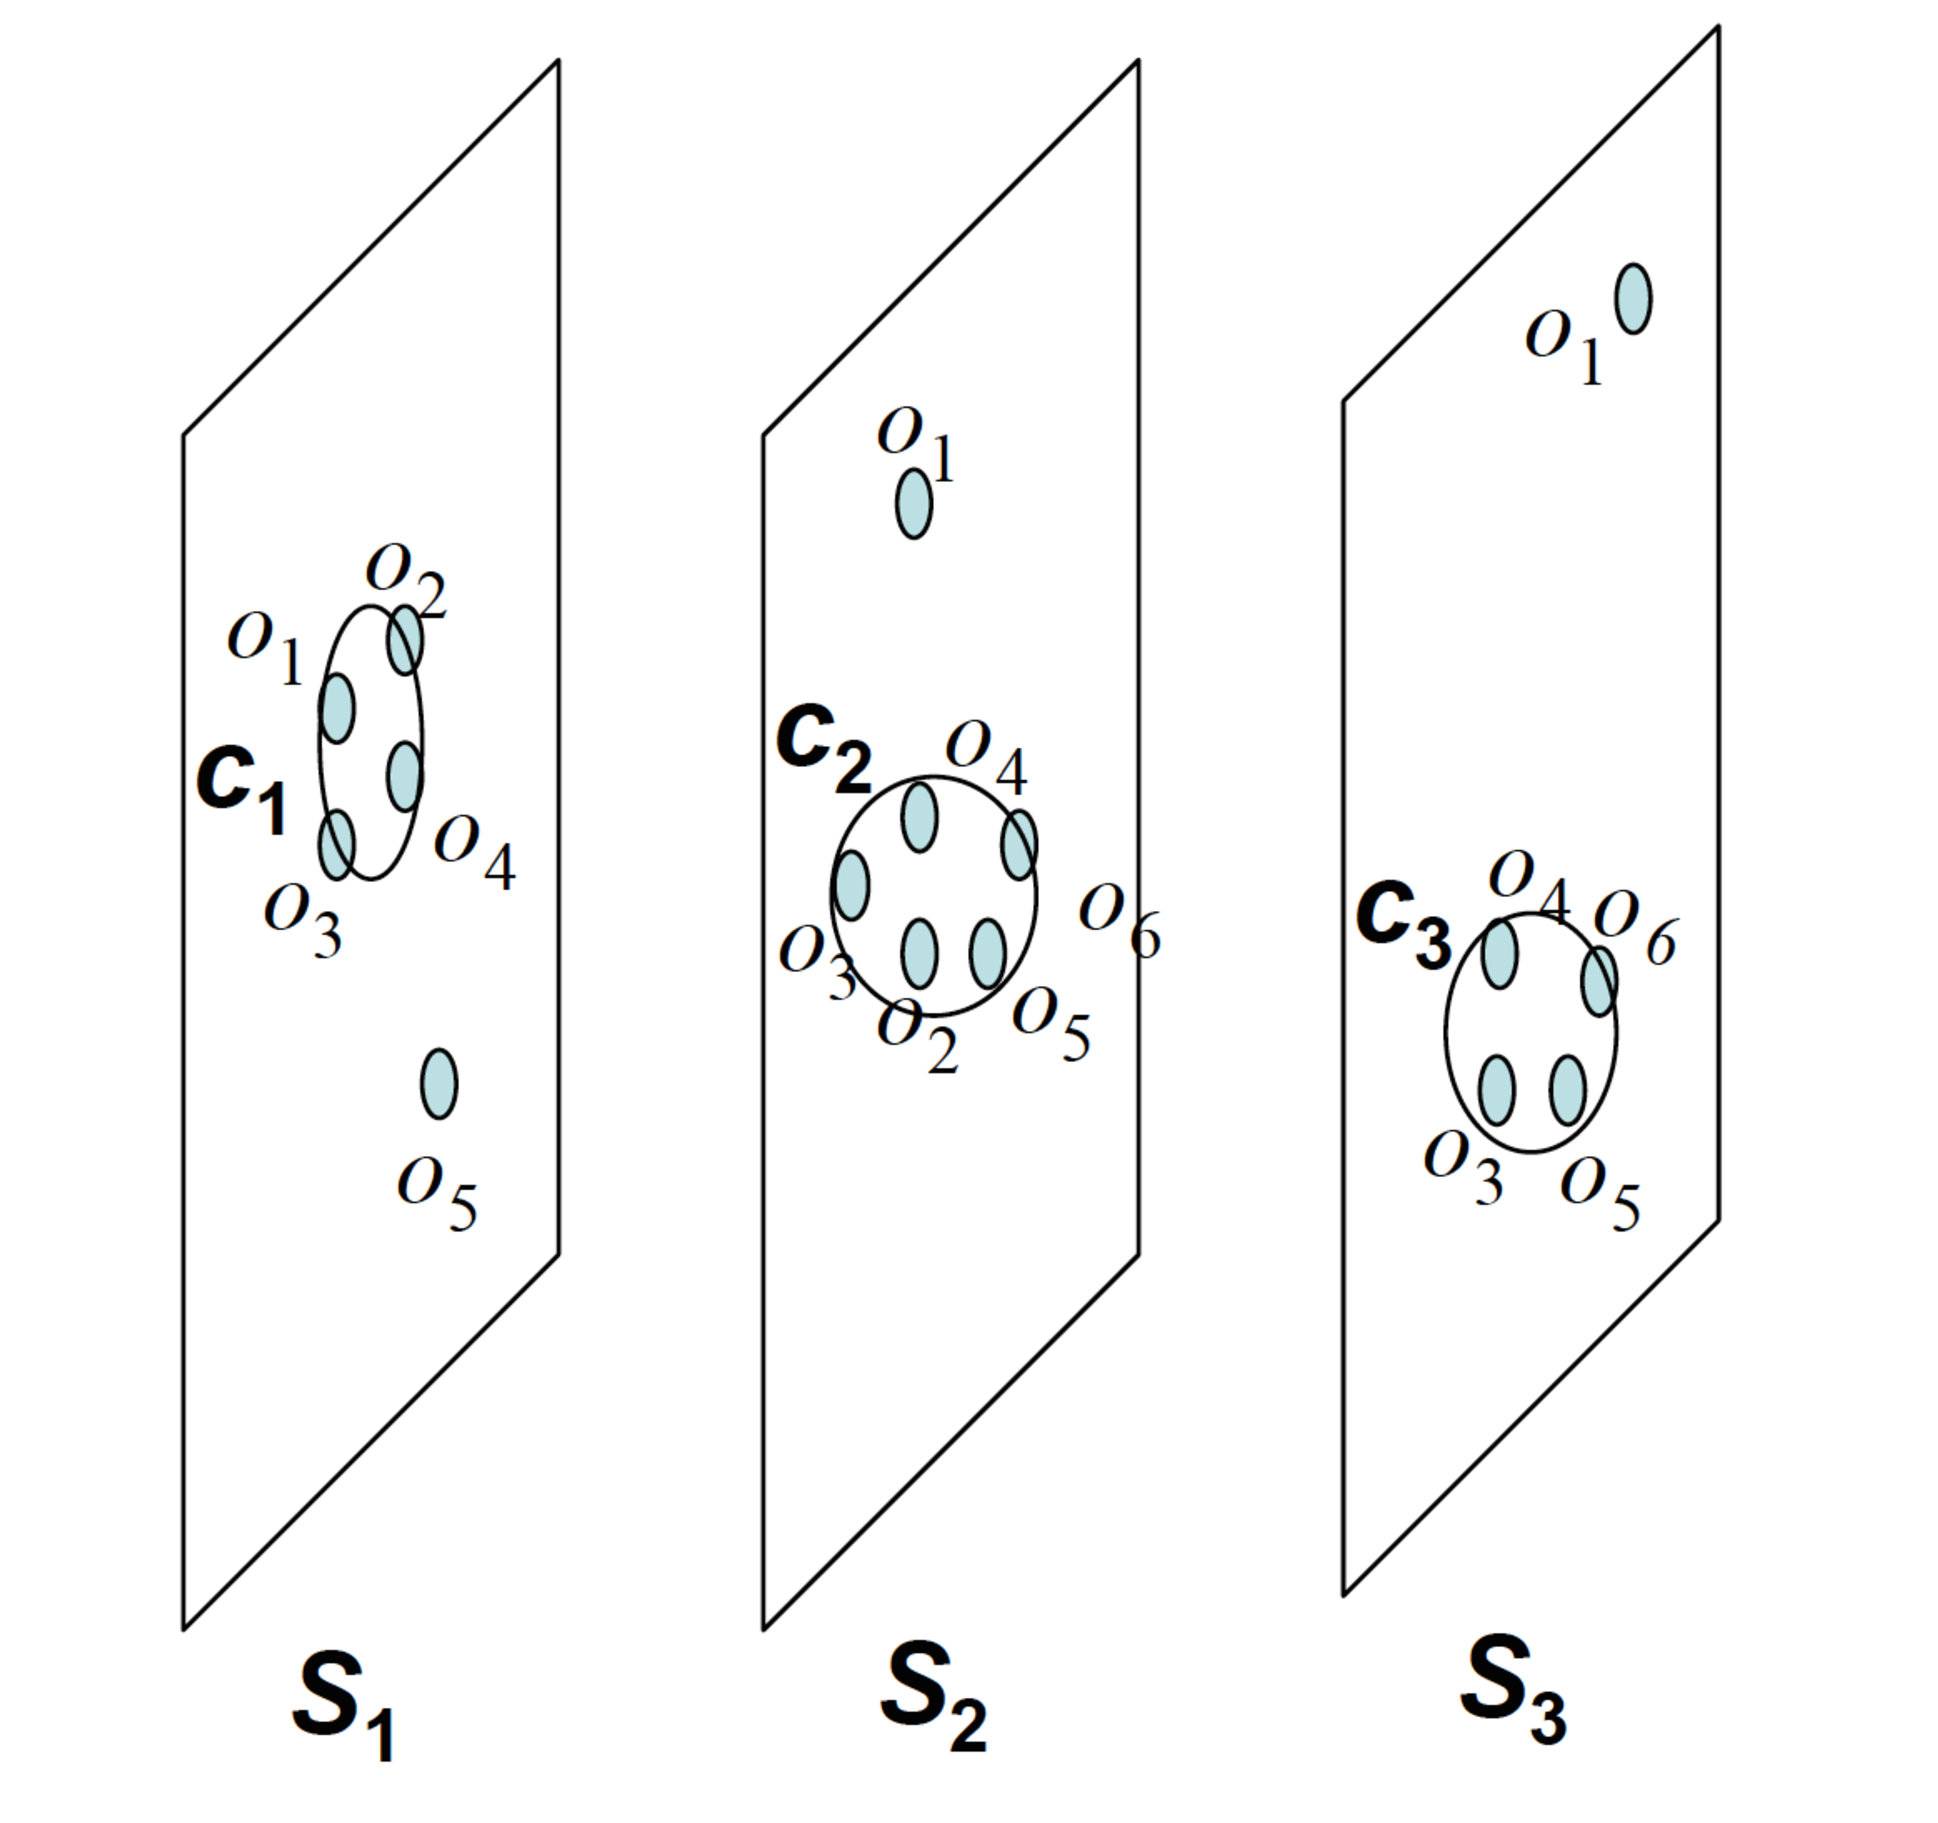
\includegraphics[width=0.5\textwidth]{images/clusters.eps}}
    \footnotesize{Source: \citep{movingclusters}.}
    \label{fig:clusters}
\end{figure}

Jeung et al. proposes the convoy pattern \citep{convoy2}\citep{convoy}. They first point out the key difference between
flock and convoy patterns: flock pattern relies on all trajectories being present in a disk of pre-defined radius, while
convoy does not rely on any kind of shape to cluster its trajectories. That difference is depicted in
\figref{fig:convoy_pattern}, where the second disk is of different size of the other disks and not all trajectories are
present in the consecutive clusters (another difference from the flock pattern). The authors propose three density based
algorithms to find convoy patterns using line simplification techniques. Their work is inspired by the algorithms
already proposed by Kalnis et al. \citep{movingclusters} and \textit{\ac{dbscan}} \citep{dbscan}. More work on convoy
patterns can be found with Aung et al. \citep{convoy3}, where they divide convoy patterns in two different groups,
namely \textit{\acp{dc}} and \textit{\acp{ec}}. To this end, they present three algorithms to identify \ac{ec} patterns.

\begin{figure}
    \centering
    \caption{A Convoy pattern}
    \centerline{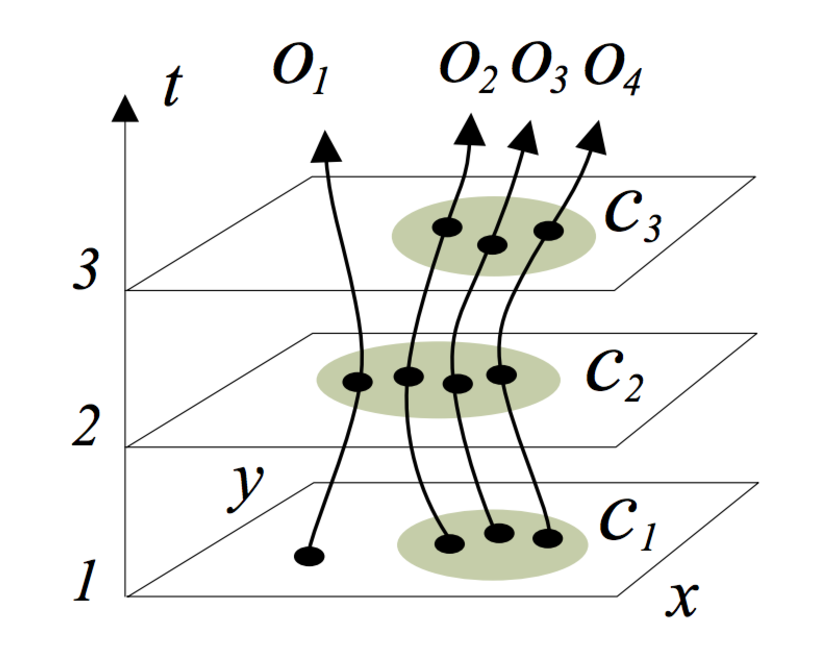
\includegraphics[width=0.5\textwidth]{images/convoy.eps}}
    \footnotesize{Source: \citep{convoy2}.}
    \label{fig:convoy_pattern}
\end{figure}

Gathering is another moving pattern that was analyzed by the academia. Zheng et al. \citep{gathering} state that a
gathering pattern consists in various grouped incidents such as celebrations, parades, protests, traffic jams, etc. They
first formalize and model the gathering pattern and then propose algorithms to find the such pattern. Effectiveness and
efficiency evaluations are presented, showing an overall good result, however only one dataset is analyzed. Instead of
looking for patterns that happen exactly at the same time (e.g. clusters and flocks), Li et al. \citep{swarm} propose
the swarm pattern. Such pattern tries to group \acp{mo} that may actually diverge temporarily and congregate at certain
timestamps, it is not required also that a trajectory stays all the time with the same swarm cluster. The authors in
that work formalize the swarm concept and present algorithms to find the pattern. The effectiveness of the algorithms
is compared against convoy pattern algorithms and it is shown that, for some datasets, the swarm pattern is better
suited.

An algorithm to find patterns in Origin-Destination databases, meaning that only the origin and destination points of a
trajectory are recorded in the analyzed dataset, is presented by Guo et al. \citep{discovering_orig_dest}. They proposed
a way to model points of interest, since \acp{mo} going to the same place (e.g. airport) will report different \ac{gps}
coordinates. The proposed algorithm has a preprocessing phase that makes a Delaunay Triangulation of the points and then
clusters those points based on two parameters: ($k$) the number of points to build a cluster and ($\theta$) the minimum
number of points (or weight) of a cluster. After building the clusters, they derive some mobility measures, in order to
extract spatial and temporal mobility patterns, presenting an useful way of understanding traffic loads in a city.

Baratchi et al. proposed a way to find frequently visited paths between two points of interests. The authors presented
an algorithm that deals with trajectory uncertainty and uses cluster based techniques to map uncertain trajectories to
actual paths in a map that were most likely to be followed by the \ac{mo}. First they gathered points of interests
(those where the \ac{mo} stayed for at least 30 minutes with its speed close to 0) and grouped all subtrajectories that
had the same start and end points of interest. They then applied their algorithm, which consists in dividing the space
in grids and assigning each point to a grid, and partitioned those subtrajectories in even small subtrajectories based
on breakpoints.  After that partition step they used a score mechanism to decide which set of subtrajctories are more
likely to be a frequent path. Their algorithm is mainly targeted for offline analyses and uses a map matching algorithm
in order to match \ac{gps} points to actual map segments. They did not present the dataset used for evaluation nor the
numbers of such dataset. Their evaluation was somewhat shallow and did not present any take away results.

A comprehensive state-of-the-art review in trajectory data mining is presented by Zheng \citep{survey}. He covered
relevant research topics, such as trajectory data preprocessing, trajectory data management, uncertainty of
trajectories, trajectory pattern mining, and trajectory classification. He pointed out some public trajectory datasets
that can be used to evaluate pattern detection algorithms, like the dataset in \citep{tdrive} used in this dissertation.

\section{Flock pattern mining}
\label{sec:rel_flocks}
Gudmundsson et al. \citep{gudefficient} \citep{gudlongest} extended and formalized the flock concept proposed by the
\ac{remo} Framework \citep{remo}. They also introduced the concept that the flock pattern must contain a disk of radius
$R$, enclosing all trajectories, in each time step. They proposed approximation and exact algorithms for flock pattern
detection, but no performance evaluations were made and only theoretical analyses were presented, which does not show if
the algorithms are efficient or not. Later on, the same authors \citep{gudlongest} extended the flock pattern definition
by adding the temporal length variable: the entities must stay together during some time interval $\delta$ to be claimed
as a flock. To this end, they presented some approximation algorithms what work on approximating the radius $R$ of the
disk used to cluster the flock, based on a defined $\epsilon$. The evaluations performed \citep{gudlongest} varied only
the $\delta$ parameter leaving all other parameters variation out of the experiments. Additionally, the performance
results were not good, having scenarios where the algorithms took more than 1500 seconds to analyze a dataset containing
1 million of entries. It is important to say that all algorithms did waste time by analyzing disks that would not form a
flock pattern, thus having a degradation in performance.

Vieira et al. \citep{vieira} proposed a polynomial algorithm to find flock patterns of fixed duration, based in three
parameters: minimum number of trajectories $\mu$, the disk radius $\epsilon$ and a minimum time length $\delta$.  In
order to discover the centers of the cluster disks for each time step, they paired the points that had distance less or
equal to $2*\epsilon$, created two disks based in that pair and tried to cluster other points into those disks. Their
algorithm assumed that each point is sampled in a fixed time interval, assumption that does not reflect real-world
datasets. Additionally, their algorithm suffered from wasting \ac{cpu} cycles by processing disk candidates that were
not real potential flock candidates. The authors also proposed some filtering heuristics to optimize the processing
time, but the optimizations did not present good results, and our local tests showed that the optimizations affected the
final number of flocks found by the algorithm.

An algorithm that mixed together \ac{bfe} \citep{vieira} with a "Frequent Pattern Mining" heuristic is proposed by
Turdukulov et al. \citep{visual}. They made some performance comparison against \ac{bfe} and were able to show some
improvement in the processing time when varying the radius $R$ of the disk. However, despite the improvements, their
results did not propose a fair comparison: (1) \ac{bfe} is an on-line algorithm and their implementation imposed an
offline implementation; (2) they filtered out some trajectories based on random assumptions, e.g. trajectories with less
than 10 minutes or 20 minutes, which might benefit their algorithm and cut out possible flocks of that length; (3) they
only showed results varying the disk radius and not the other parameters used by \ac{bfe}.

The problem of \ac{mfp} is addressed by the work of Geng et al. \citep{enumeration}, which proposed algorithms to
enumerate all \ac{mfp} in a trajectory dataset. \ac{mfp}, in other words, means that the flock cannot be extended
without increasing the disk radius $R$. They proposed a set of algorithms for finding \ac{mfp} and proved that they
could indeed enumerate all \ac{mfp} from a trajectory dataset. They also compared their algorithms with \ac{bfe} from
Vieira et al. \citep{vieira} and showed that their implementations outperformed the later in some scenarios. However,
they still wasted \ac{cpu} cycles by analyzing disks that would be discarded later, by not being potential flock
candidates.

Wachowicz et al. \citep{flockpedestrian} and Wirz et al. \citep{pedestriancanyons} presented algorithms for finding
flocks using pedestrian spatio-temporal data. The former performed a lot pre- and post-processing in the dataset (which
makes not possible to be used in real-time analysis) and neither performance nor accuracy evaluations were presented.
The latter, did not provide any performance evaluation either, only showing accuracy experiments with a tiny dataset of
only 13 entities in a time span of 32 minutes.

Wang et al. \citep{visualtrafficjam} proposed a framework for detecting traffic jams in trajectory data, which can be
considered as a flock pattern, since \acp{mo} stay together in a road during an interval of time. They listed the
requirements for both a data model and a visual interface for their system, in order to be able to expose useful
information for users and extract conclusions from the analysis. Their algorithm was bound to a map network, which means
that one part of data preprocessing would be to map the data points to the respective roads in a map. They claimed to be
able to detect traffic jams with high accuracy, however they did not have any ground truth data to validate the
assumptions. It is also worth noting that only one dataset was used to evaluate the proposed system, which did not show
that the solution was ready for varied data scenarios.

There were also some studies focusing on indoor flock detection using mobile phone sensors, in which Wi-Fi signal
strengths were mapped into coordinates \citep{mobile1}, or a variety of mobile phone sensors (e.g. accelerometer,
magnetometer and Wi-Fi) were used to detect flock patterns \citep{mobile2}. However, those studies only addressed flock
detection in indoor environments, not using \ac{gps} coordinates, which are not in the scope of the problem addressed by
this dissertation.

\section{Academic Contribution}
It is notorious, from the related work presented in \secref{sec:rel_general} and \secref{sec:rel_flocks}, that there is
a lot to cover in order to provide efficient flock pattern detection as well as a lack of elegant and modular System
Architecture to address the flock pattern detection problem (which was not seen in any of the presented works). All of
that is a subject to care about due to the extensive number of scenarios that data pattern mining, as well as flock
patterns, can help and be applied to. We can have flock pattern detection helping the following, to name a few
\citep{applications}:

\begin{enumerate}
    \item \textbf{Traffic Management}: Unusual grouping of vehicles, or abnormal traffic volume in certain regions can
        be detected with the help of flock pattern detection algorithms. That information can help the accountable
        entities to better plan cities or traffic spaces.
    \item \textbf{Surveillance and Security}: Suspicious movements of groups of people or vehicles can indicate a
        security threat and automatic pattern detection systems can aid the detection of abnormal behavior in a group of
        \acp{mo}.
    \item \textbf{Human Movement}: Governmental organizations can study how people are moving from one part of the
        city/country/state to another with the help of flock pattern detection. They can also acquire information about
        the habits of the population and provide resources to enhance life quality of those involved.
\end{enumerate}

In \secref{sec:architecture} we will propose an elegant, modular and simple System Architecture that will be able
address flock pattern detection problems. Such architecture will be divided in logic modules and components, each one
with a very specific and self-contained goal, making then reusable and good candidates to address other data analysis
problems. We will also show that by modifying a single component in that architecture will enable the usage of a
different software paradigm, thus proving its modularity, extensibility and ease of use.

We could notice that the presented algorithms suffer from \ac{cpu} cycles waste by processing data that will not
generate any pattern, like the flock disks that contain points that are not present in subsequent time steps. Avoiding
such unnecessary processing can boost the running time of a flock pattern detection algorithm and then provide
information in a real-time fashion for decision takers. With that in mind, we will present an efficient algorithm, based
on bitmaps, that will only be concerned with data that can really generate flock patterns, saving a considerable amount
of time. Moreover, our algorithm will be able to provide information, about the datasets being analyzed, way faster than
other algorithms. We will prove such efficiency by showing benchmarks comparing the running time of our solution against
the state-of-the-art algorithm and also show how that our implementation generates way less unimportant data than the
comparison target algorithm, which dramatically affects the running time of the latter. Last, but not least, we will
provide a multi-core aware implementation of our algorithm, taking advantage of the proposed system architecture
mentioned in the previous paragraph, which will achieve even more savings in running time, without affecting the number
of flocks that are found.  Aiming at showing that our solution is ready for multiple types of data, we will perform
experiments with 4 different datasets, being them real and synthetic generated and with a large amount of data entries,
with some of them having more then 50 million records.
